\section{Basic Concepts}

\begin{frame}{What is Frequent-pattern Analysis?}
	\begin{itemize}
		\item \textbf{Frequent pattern:}
		      \begin{itemize}
			      \item A pattern (a set of items, subsequences, substructures, etc.)
			            that occurs frequently in a dataset.
		      \end{itemize}
		\item \textbf{Motivation: Finding inherent regularities in data:}
		      \begin{itemize}
			      \item What products are often purchased together? Beer and diapers?!
			      \item What are the subsequent purchases after buying a PC?
			      \item Who bought this has often also bought $\ldots$"
			      \item What kinds of DNA are sensitive to this new drug?
			      \item Can we automatically classify Web documents?
		      \end{itemize}
		\item \textbf{Applications:}
		      \begin{itemize}
			      \item Basket-data analysis, cross-marketing, catalog design,
			            sale-campaign analysis, Web-log (click-stream) analysis, and
			            DNA-sequence analysis.
		      \end{itemize}
	\end{itemize}
\end{frame}

\begin{frame}{Why is Frequent-pattern Mining Important?}
	\begin{itemize}
		\item \textbf{A frequent pattern is an intrinsic and important property
			      of a dataset.}
		\item \textbf{Foundation for many essential data-mining tasks:}
		      \begin{itemize}
			      \item Association, correlation, and causality analysis.
			      \item Sequential, structural (e.g., sub-graph) patterns.
			      \item Pattern analysis in spatiotemporal, multimedia, time-series,
			            and stream data.
			      \item Classification: discriminative, frequent-pattern analysis.
			      \item Cluster analysis: frequent-pattern-based clustering.
			      \item Data warehousing: iceberg cube and cube gradient.
			      \item Semantic data compression: fascicles (Jagadish, Madar, and
			            Ng, VLDB'99).
			      \item Broad applications.
		      \end{itemize}
	\end{itemize}
\end{frame}

\begin{frame}
	\frametitle{Some Real World Examples}

	\begin{center}
		\begin{tikzpicture}
			\node at (7,-2) [inner sep=0pt, opacity=0] {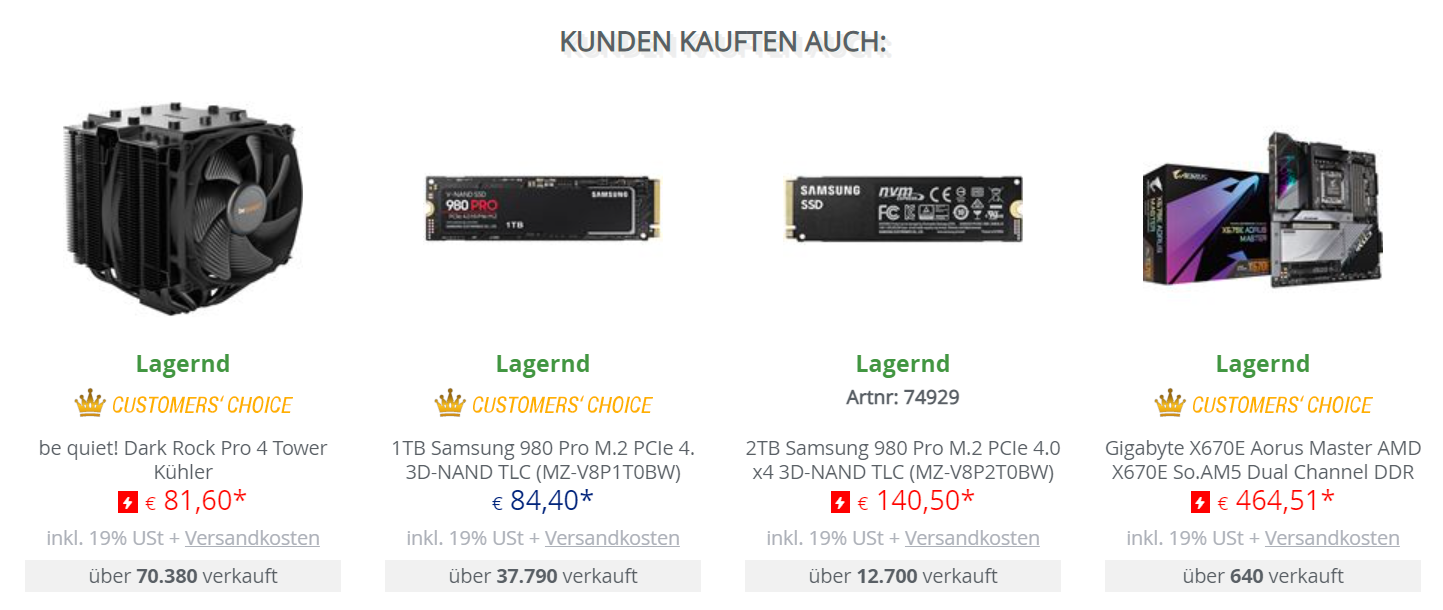
\includegraphics[height=0.4\textheight]{img/frequent-patterns-mindfactory.png}}; % Invisible node
			\node<1-> (img1) at (0,0) [inner sep=0pt, blur shadow={shadow blur steps=20, shadow xshift=0.1ex, shadow yshift=-0.1ex}] {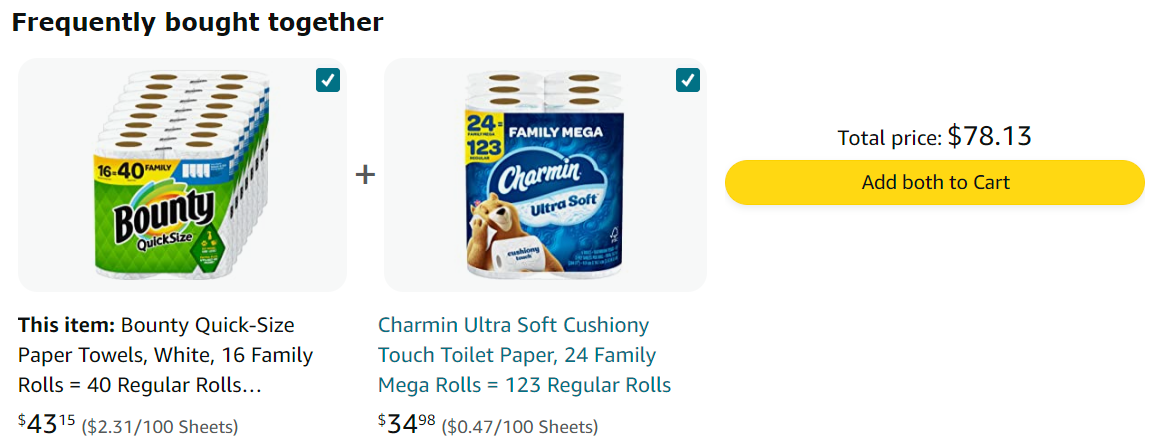
\includegraphics[height=0.4\textheight]{img/frequent-patterns-amazon.png}};
			%\node<1-> at (img1.south) [yshift=-0.5cm] {\scriptsize Amazon};
			\node<2-> (img2) at (3.5,-1) [inner sep=0pt, blur shadow={shadow blur steps=20, shadow xshift=0.1ex, shadow yshift=-0.1ex}] {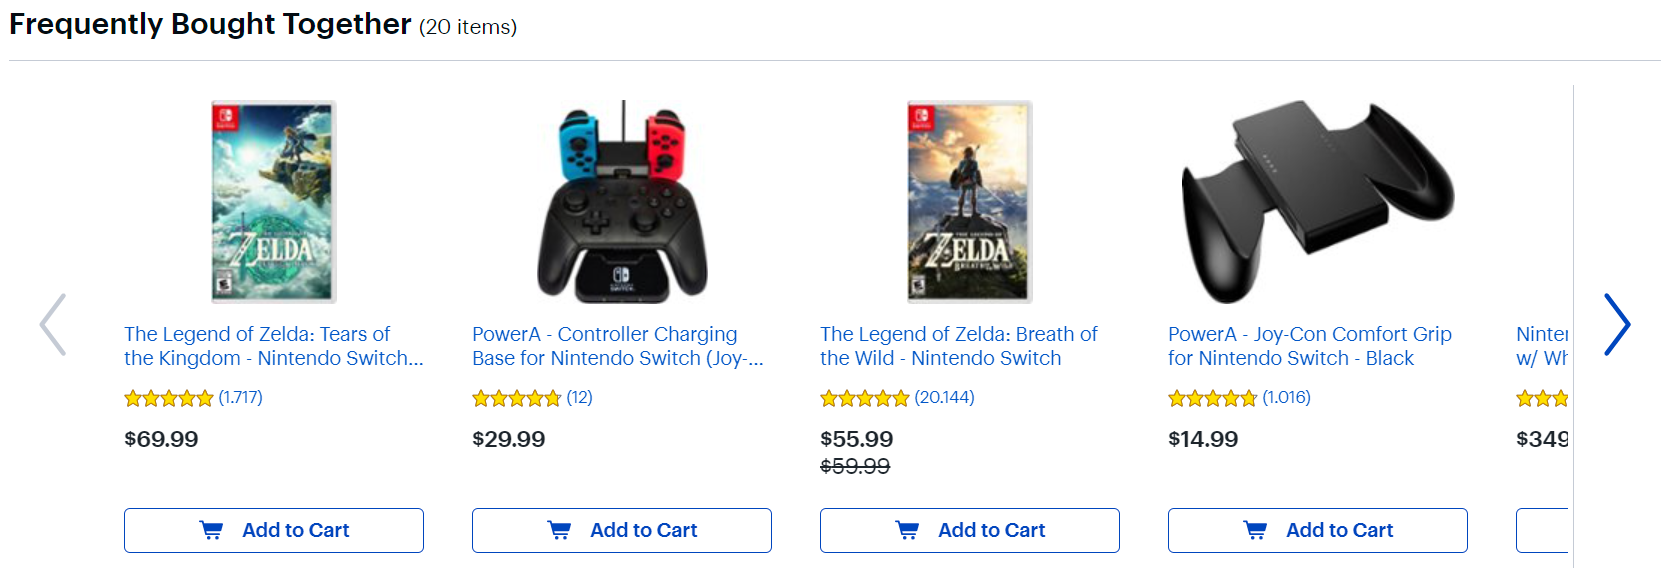
\includegraphics[height=0.4\textheight]{img/frequent-patterns-bestbuy.png}};
			%\node<2-> at (img2.south) [yshift=-0.5cm] {\scriptsize Best Buy};
			\node<3-> (img3) at (7,-2) [inner sep=0pt, blur shadow={shadow blur steps=20, shadow xshift=0.1ex, shadow yshift=-0.1ex}] {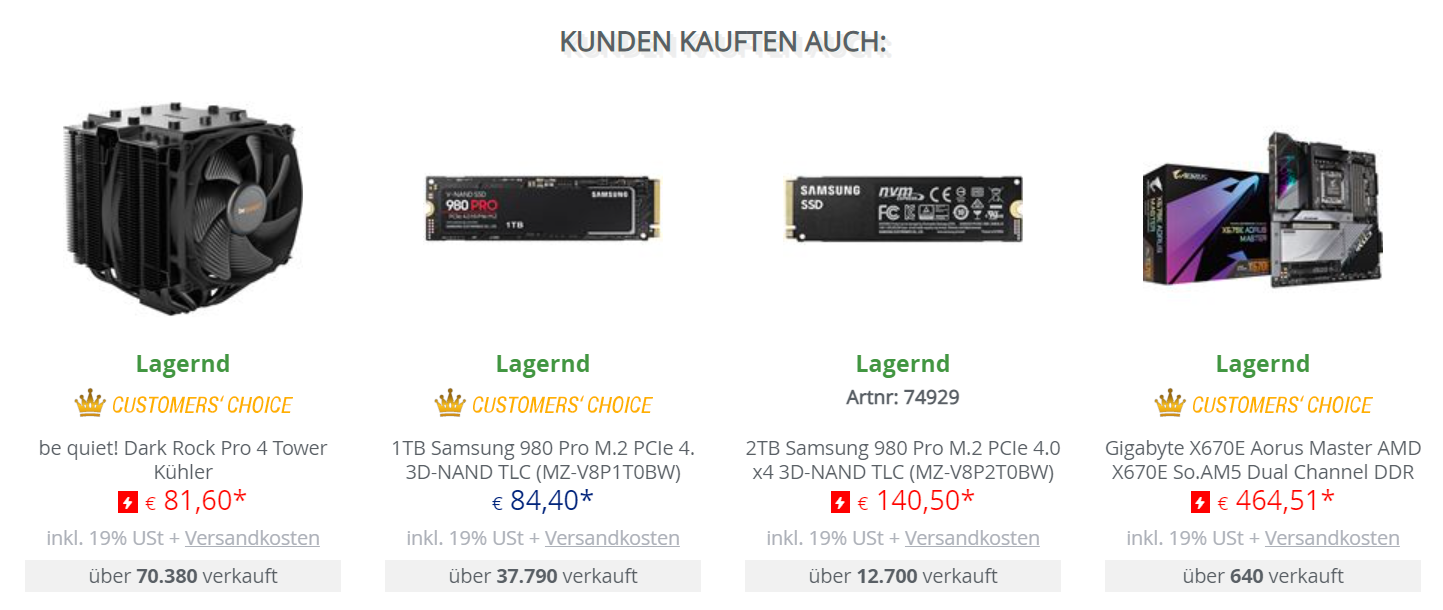
\includegraphics[height=0.4\textheight]{img/frequent-patterns-mindfactory.png}};
			%\node<3-> at (img3.south) [yshift=-0.5cm] {\scriptsize Mindfactory};
		\end{tikzpicture}
	\end{center}

\end{frame}

\begin{frame}{An Theoretical Example (I)}
	\begin{columns}
		\begin{column}{0.4\textwidth}
			\begin{tabular}{|c|c|}
				\hline
				\textbf{TID} & \textbf{Items bought}             \\\hline
				10           & Beer, Nuts, Diapers               \\\hline
				20           & Beer, Coffee, Diapers             \\\hline
				30           & Beer, Diapers, Eggs               \\\hline
				40           & Nuts, Eggs, Milk                  \\\hline
				50           & Nuts, Coffee, Diapers, Eggs, Milk \\\hline
			\end{tabular}
			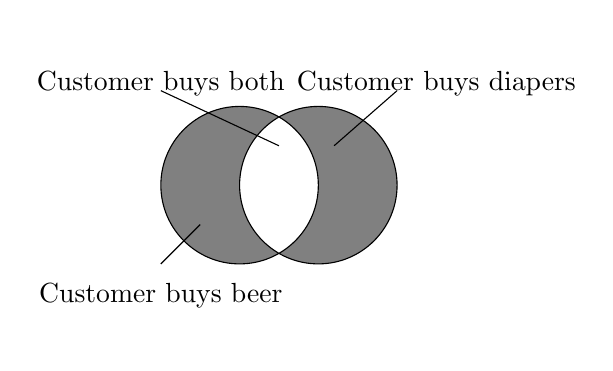
\begin{tikzpicture}[fill=gray]
				% left hand
				\scope
				\clip (-2,-2) rectangle (2,2)
				(1,0) circle (1);
				\fill (0,0) circle (1);
				\endscope
				% right hand
				\scope
				\clip (-2,-2) rectangle (2,2)
				(0,0) circle (1);
				\fill (1,0) circle (1);
				\endscope
				% outline
				\draw (0,0) circle (1) (0,1) (1,0) circle (1) (1,1);
				\node[label=below:{Customer buys beer}] at (-1,-1) {};
				\node[label=below:{Customer buys diapers}] at (2.5,1.7) {};
				\node[label=below:{Customer buys both}] at (-1,1.7) {};
				\draw (-1,-1) -- (-0.5,-0.5);
				\draw (2,1.2) -- (1.2,0.5);
				\draw (-1,1.2) -- (0.5,0.5);
			\end{tikzpicture}
		\end{column}
		\begin{column}{0.5\textwidth}
			\vspace{-2cm}
			\begin{itemize}
				\item \textbf{Itemset:}
				      \begin{itemize}
					      \item A set of one or more items.
					      \item $k$-itemset $X = \{x_1, x_2, \ldots, x_k\}$.
				      \end{itemize}
				\item \textbf{(Absolute) Support, or support count of $X$:}
				      \begin{itemize}
					      \item Frequency or occurrence of $X$.
				      \end{itemize}
				\item (Relative) Support $s$:
				      \begin{itemize}
					      \item The fraction of the transactions that contain $X$.
					      \item I.e. the \textbf{probability} that a transaction
					            contains $X$.
				      \end{itemize}
				\item \textbf{An itemset $X$ is frequent, if $X$'s support is
					      no less than a \texttt{min\_sup} threshold.}
			\end{itemize}
		\end{column}
	\end{columns}
\end{frame}

\begin{frame}{An Theoretical Example (II)}
	\begin{columns}
		\begin{column}{0.4\textwidth}
			\begin{tabular}{|c|c|}
				\hline
				\textbf{TID} & \textbf{Items bought}             \\\hline
				10           & Beer, Nuts, Diapers               \\\hline
				20           & Beer, Coffee, Diapers             \\\hline
				30           & Beer, Diapers, Eggs               \\\hline
				40           & Nuts, Eggs, Milk                  \\\hline
				50           & Nuts, Coffee, Diapers, Eggs, Milk \\\hline
			\end{tabular}
			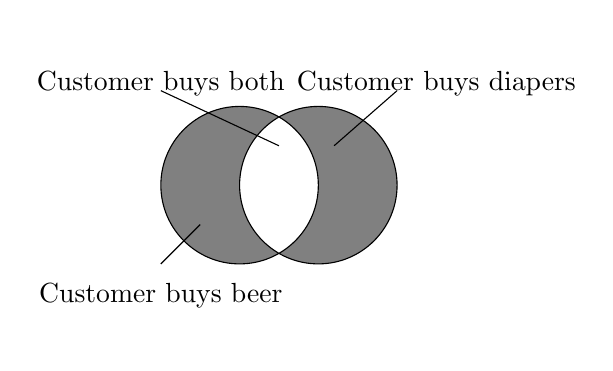
\begin{tikzpicture}[fill=gray]
				% left hand
				\scope
				\clip (-2,-2) rectangle (2,2)
				(1,0) circle (1);
				\fill (0,0) circle (1);
				\endscope
				% right hand
				\scope
				\clip (-2,-2) rectangle (2,2)
				(0,0) circle (1);
				\fill (1,0) circle (1);
				\endscope
				% outline
				\draw (0,0) circle (1) (0,1) (1,0) circle (1) (1,1);
				\node[label=below:{Customer buys beer}] at (-1,-1) {};
				\node[label=below:{Customer buys diapers}] at (2.5,1.7) {};
				\node[label=below:{Customer buys both}] at (-1,1.7) {};
				\draw (-1,-1) -- (-0.5,-0.5);
				\draw (2,1.2) -- (1.2,0.5);
				\draw (-1,1.2) -- (0.5,0.5);
			\end{tikzpicture}
		\end{column}
		\begin{column}{0.5\textwidth}
			\vspace{-2cm}
			\begin{itemize}
				\item \textbf{Find all the rules $X \implies Y$ with minimum
					      support and confidence.}
				      \begin{itemize}
					      \item \textbf{Support} $s$: probability that a transaction
					            contains $X \cup Y$.
					      \item \textbf{Confidence} $c$: conditional probability that
					            a transaction having $X$ also contains $Y$.
				      \end{itemize}
				\item \textbf{Example:}
				      \begin{itemize}
					      \item $\text{min\_sup} = 50\%$ and $\text{min\_conf} =
						            50\%$.
					      \item Frequent itemsets:
					            \begin{itemize}
						            \item Beer: $3$, Nuts: $3$, Diapers: $4$, Eggs: $3$,
						                  $\{\text{Beer, Diapers}\}$: $3$.
					            \end{itemize}
					      \item \textbf{Association rules:}
					            \begin{itemize}
						            \item Beer $\implies$ Diapers ($60\%$, $100\%$).
						            \item Diapers $\implies$ Beer ($60\%$, $75\%$).
					            \end{itemize}
				      \end{itemize}
			\end{itemize}
		\end{column}
	\end{columns}
\end{frame}

\begin{frame}{Basic Concepts: Association Rules}
	\begin{itemize}
		\item \textbf{Implication of the form $A \implies B$:}
		      \begin{itemize}
			      \item where $A \neq \emptyset$, $B \neq \emptyset$ and $A \cap B =
				            \emptyset$.
		      \end{itemize}
		\item \textbf{Strong rule:}
		      \begin{itemize}
			      \item Satisfies both $\text{min\_sup}$ and $\text{min\_conf}$
			            \begin{align*}
				            \text{support}(A \implies B)    & = P(A \cup B),                                        \\
				            \text{confidence}(A \implies B) & = P(B | A)                                            \\
				                                            & = \frac{\text{support}(A \cup B)}{\text{support}(A)}.
			            \end{align*}
			      \item I.e. confidence of rule can be easily derived from the
			            support counts of $A$ and $A \cup B$.
		      \end{itemize}
		\item \textbf{Association-rule mining:}
		      \begin{itemize}
			      \item Find all frequent itemsets.
			      \item Generate strong association rules from the frequent itemsets.
		      \end{itemize}
	\end{itemize}
\end{frame}

\begin{frame}{Closed Itemsets and Max-itemsets (I)}
	\begin{itemize}
		\item \textbf{A long itemset contains a combinatorial number of
			      sub-itemsets.}
		      \begin{itemize}
			      \item E.g. $\{a_1,a_2,\ldots,a_{100}\}$ contains
			            \begin{align*}
				            {100\choose 1} + {100 \choose 2} + \cdots + {100 \choose 100} =
				            2^{100}-1 \approx 1.27 \cdot 10^{30} \; \text{sub-itemsets!}
			            \end{align*}
			      \item \textbf{Solution:}
			            \begin{itemize}
				            \item Mine closed itemsets and max-itemsets instead.
			            \end{itemize}
			      \item \textbf{An itemset $X$ is closed, if $X$ is frequent and
				            there exists no super-itemset $X \subset Y$ with the same support
				            as $X$.} (Pasquier et al., ICDT'99)
			      \item \textbf{An itemset $X$ is a max-itemset, if $X$ is frequent
				            and there exists no frequent super-itemset $X \subset Y$.}
			            (Bayardo, SIGMOD'98)
			      \item \textbf{Closed itemset is a lossless "compression" of
				            frequent itemsets.}
			            \begin{itemize}
				            \item Reducing the number of itemsets (and rules).
			            \end{itemize}
		      \end{itemize}
	\end{itemize}
\end{frame}

\begin{frame}{Closed Itemsets and Max-itemsets (II)}
	\begin{itemize}
		\item \textbf{Example:}
		      \begin{itemize}
			      \item $\text{DB} = \{\langle a_1,a_2, \ldots, a_{100} \rangle,
				            \langle a_1, a_2, \ldots, a_{50} \rangle \}$.
			      \item I.e. just two transactions.
			      \item $\text{min\_sup} = 1$.
		      \end{itemize}
		\item \textbf{What are the closed itemsets?}
		      \begin{itemize}
			      \item $\langle a_1,a_2, \ldots, a_{100} \rangle : 1$,
			      \item $\langle a_1,a_2, \ldots, a_{50} \rangle : 2$,
			      \item Number behind the colon: support\_count.
		      \end{itemize}
		\item \textbf{What are the max-itemsets?}
		      \begin{itemize}
			      \item $\langle a_1,a_2, \ldots, a_{100} \rangle : 1$.
		      \end{itemize}
		\item \textbf{What is the set of all frequent itemsets?}
	\end{itemize}
\end{frame}
